\newchapter{Musket Ball: Observed Properties}{Musket Ball Cluster: Observed Properties}{Musket Ball Cluster: Observed Properties}
\label{chapter:2}

\noindent This chapter is an expanded version of the article titled \emph{Discovery of a Dissociative Galaxy Cluster Merger with Large Physical Separation} which was published in the March 2012 issue of the Astrophysical Journal Letters (Volume 747, pp. L42). \\

We present DLSCL J0916.2+2951 ($z$=0.53), a major cluster merger in which the collisional cluster gas has become dissociated from the collisionless galaxies and dark matter.
We identified the cluster using optical and weak lensing observations as part of the Deep Lens Survey. 
Our follow-up observations with {\it Keck}, {\it Subaru}, {\it Hubble Space Telescope}, and {\it Chandra} show that the cluster is a dissociative merger.


\section{Introduction}

We have identified a new dissociative merger, DLSCL J0916.2+2951, that probes an unexplored area of merger phase-space.  
We originally detected the cluster in the Deep Lens Survey \citep[DLS;][]{Wittman:2002cp} via its weak lensing (WL) shear signal. 
It consists of two main subclusters  spectroscopically confirmed to be at the same redshift (0.53).
This cluster was also observed in the Sunyaev-Zel'dovich Array Survey \citep{Muchovej:2010gc} which provided evidence that the cluster gas is dissociated from the bulk of the mass and galaxies (Figure \ref{figure:MusketBallSZ}).
Follow-up optical observations with {\it Subaru} and {\it HST} enable higher resolution mass maps and follow-up X-ray observations with {\it Chandra} ACIS-I confirm that the majority of the gas is offset between the North and South subclusters, the signature of a dissociative merger (Figure \ref{fig1}).

In this chapter we introduce DLSCL J0916.2+2951 and summarize our survey of its three dominant components (galaxies, DM, and gas) and the cluster's astrophysical implications.
A more thorough exposition of the survey and analysis will be presented in Dawson et al. (in preparation).
Throughout this dissertation we assume $\Omega_{\Lambda}=0.7$, $\Omega_m=0.3$, and $H=70$\,km\,s$^{-1}$\,Mpc$^{-1}$.

\begin{figure}
\plotone{Chapter2/fig1.png}
\caption[Merging cluster DLSCL J0916.2+2951 and its three matter components.]{Merging cluster DLSCL J0916.2+2951 and its three matter components. 
Overlaid on the HST color image of the galaxies is the total mass distribution (blue) based on WL analysis of the HST images and the cluster gas distribution (red) based on Chandra X-ray observations.  
The bulk of the collisional gas is located between the two collisionless galaxy and mass concentrations, indicative of a dissociative merger. 
The image is $5\arcmin \times 5\arcmin$ ($\sim 1.9\times 1.9$\,Mpc$^2$ at $z=0.53$).\label{fig1}}
\end{figure}

\section{Photometric Studies}

We obtained $B,V,R,$ and $z'$ photometric data (12, 12, 18, and 12\,ksec, respectively) with Mosaic 1 on the KPNO 4-m {\it Mayall} telescope as part of the DLS.
To improve the accuracy of our photometric redshifts we also observed the cluster in three medium-width optical bands ($g,h,$ and $i$ from the BATC filter set), bracketing the redshifted $4000$\,\AA\, feature, using the upgraded Mosaic 1.1 imager on the KPNO {\it Mayall} with exposure times of 6\,ks per filter (2011 April 22--24).
We estimate colors using \emph{ColorPro} \citep{Coe:2006jf} and redshifts using \emph{BPZ} \citep{Benitez:2000jr}.
We replace the standard templates with a set ``tweaked'' in a method similar to that described in \citet{Ilbert:2006bw}, using spectroscopic samples from SHELS \citep{Geller:2005dj} and the PRIMUS survey \citep{Coil:2010to} which overlap the DLS.
Figure \ref{fig2} shows the density isopleths of galaxies with $0.43<z_{\rm phot}<0.63$ (roughly the cluster redshift $\pm\sigma_{z_{\rm phot}}$).
This map agrees well with the distribution of spectroscopically confirmed cluster members.

\begin{figure}
%\epsscale{1.06}
\plottwo{Chapter2/fig2a.png}{Chapter2/fig2b.png}
\caption[Color image of DLSCL J0916.2+2951 and its galaxy number density with a histogram of the spectroscopic redshifts in the area.]{\emph{Left:} DLS composite $BVR$ color image of DLSCL J0916.2+2951 showing  the galaxies of the two subclusters. The white contours represent the number density of galaxies with $z_{\rm phot}=0.53\pm0.1$, the cluster redshift $\pm\sigma_{z_{\rm phot}}$. The contours begin at 200 galaxies\,Mpc$^{-2}$ with increments of 50 galaxies\,Mpc$^{-2}$. 
The image field-of-view is the same as Figure \ref{fig1}.
\emph{Right:} Histogram of the 200 observed spectroscopic redshifts within the field of view of the \emph{left} figure.  The red portion is the subsample that passes the $z_{\rm phot}=0.53\pm0.1$ criteria. The galaxies at $z\sim0.6$ had equal probability of selection as the cluster members and show no sign of clustering. 
\label{fig2}}
\end{figure}

\section{Spectroscopic Studies}\label{section:MusketBallSpectroscopy}

We obtained spectroscopic redshifts for 20 cluster members with {\it Keck} LRIS (2007 January 16) and 634 unique spectroscopic redshifts (0\,$<$\,$z$\,$<$\,1.2)  in a $\sim15\arcmin\times 15\arcmin$ area centered on the cluster with {\it Keck} DEIMOS (2011 March 2--3), including 132 members at the cluster redshift.
We reduced the LRIS spectra using a scripted sequence of standard IRAF reduction tasks, and the DEIMOS spectra using a modified version of the DEEP2 \emph{spec2d} package \citep{Davis:2003fe,Gal:2008bg,Lemaux:2009fy}.

We use our full sample of 654 spectroscopic redshifts as well as photometric redshifts to identify potential line-of-sight structures which may confuse our results.
We find no evidence for significant line-of-sight structure (Figure \ref{fig2}).

We estimate each subcluster's redshift and velocity dispersion (Table \ref{tbl1}) using the biweight-statistic and bias-corrected 68\% confidence limit \citep{Beers:1990kg} applied to 100,000 bootstrap samples of each subcluster's spectroscopic redshifts.
Our redshift estimates indicate a line-of-sight velocity difference of $v_{\rm los}=670^{+270}_{-330}$ km s$^{-1}$ between the North and South subclusters, using the galaxies within a 0.5\,Mpc radius centered on the {\it HST} WL mass peaks and within a velocity range of $\pm 3000$\,km\,s$^{-1}$ of $z$=0.53 ($\sim3\times$ the expected velocity dispersion); corresponding to 38 and 35 galaxies for the North and South subcusters, respectively.
These results are robust against varying the velocity range $\pm1000$\,km\,s$^{-1}$ and using the Subaru WL or galaxy number density peaks as the apertures' centers, provided the aperture radius is $\lesssim$0.5\,Mpc: larger radii lead to significant subcluster membership confusion.
Additionally, we report the velocity dispersion mass estimates based on the scaling relation of \citet{Evrard:2008jm} in Table \ref{tbl1}.
We note that the velocity dispersions should be interpreted with caution since this is a disturbed system.

\begin{deluxetable}{lcccccccc}
\tablewidth{0pt}
\tabletypesize{\scriptsize}
\tablecaption{Observed subcluster and X-ray concentration properties\label{tbl1}}

\tablehead{
\colhead{Subcluster}     & \colhead{Redshift}  &
 \colhead{$\sigma_v$}    &  \colhead{$\sigma_v$ M$_{200}$}&
\colhead{WL M$_{200}$}          &
\colhead{L$_{\rm X_{\rm 0.5-2keV}}$}  & \colhead{T$_{\rm X}$}  &
\colhead{X-ray} & \colhead{Joint WL}\\
\colhead{}         &  \colhead{}  &
\colhead{(km s$^{-1}$)}    &   \colhead{($10^{14}$M$_\sun$)}  & 
\colhead{($10^{14}$M$_\sun$)}          &
\colhead{($10^{43}$erg\,s$^{-1}$)}  & \colhead{(keV)}  &
\colhead{S/N} & \colhead{S/N} 
}
\startdata
North & $0.53074^{+0.00068}_{-0.00064}$ & 
 $740^{+130}_{-190}$ &
 $3.7\pm2.3$& $1.7^{+2.0}_{-0.72}$ &
0.63 & \nodata &
 3.2 & 3.0 \\
South  & $0.53414^{+0.00065}_{-0.00064}$ & 
 $770^{+110}_{-92}$ & 
 $4.1\pm1.6$& $3.1^{+1.2}_{-0.79}$ &
2.1 & $2.7^{+1.2}_{-0.7}$ &
7.0 & 6.7\\
Central & \nodata & 
\nodata & \nodata & 
\nodata &
2.8 & $2.2^{+1.4}_{-0.6}$ &
9.1 & -3.3\tablenotemark{a}\\ 
\enddata
%% Text for table notes should follow after the \enddata but before
%% the \end{deluxetable}. Make sure there is at least one \tablenotemark
%% in the table for each \tablenotetext.
\tablenotetext{a}{The negative WL S/N indicates a projected surface mass local under-density.}
%\tablecomments{Table \ref{tbl-1} is published in its entirety in the 
%electronic edition of the {\it Astrophysical Journal}.  A portion is 
%shown here for guidance regarding its form and content.}
%\tablenotetext{a}{Sample footnote for table~\ref{tbl-1} that was generated
%with the deluxetable environment}
%\tablenotetext{b}{Another sample footnote for table~\ref{tbl-1}}
\end{deluxetable}

\section{Weak Lensing Analysis}\label{section:Chap2WL}

To map the total mass distribution we use a version of the \citet{Fischer:1997ct} method modified to include a novel tomographic signal-matched filter.
The cluster's WL shear signal, $\gamma$, depends not only on the projected surface mass over-density of the cluster, $\Delta\Sigma$, but on the relative distances of the observer, the mass, and the background galaxies:
\begin{equation}
\gamma=\frac{\Delta\Sigma}{\Sigma_{cr}}=\frac{\Delta\Sigma4\pi G}{c^2}\frac{D_{ls}(z_l,z_s)D_l(z_l)}{D_s(z_s)}\mathcal{H}\left(\frac{z_s}{z_l}-1\right),
\end{equation}\label{equation:WLshear}
%\begin{displaymath}
%\gamma \propto \frac{\Delta\Sigma}{\Sigma_{cr}} = \Delta\Sigma \frac{4\pi G}{c^2} \frac{D_{ls}(z_l,z_s)D_l(z_l)}{D_s(z_s)} \mathcal{H}\left(\frac{z_s}{z_l}-1\right),
%\end{displaymath}
where $\Sigma_{\rm cr}$ is the critical surface density, $\mathcal{H}$ is the Heaviside step function,  and $D_l$, $D_s$, \& $D_{ls}$ are the angular diameter distances to the lens, source, and between the lens and source, respectively.
In addition to weights based on shape measurement errors, we also weight by each galaxy's photometric redshift probability distribution function, $p(z)$,
\begin{displaymath}
w_{\gamma}(z_l) = \Sigma_{cr}^{-1}(z_l)\approx\langle\Sigma_{cr}^{-1}(z_l)\rangle=\int\Sigma_{cr}^{-1}( z_l,z_s)p(z_s)\mathcal{H}\left(\frac{z_s}{z_l}-1\right)dz_s.
\end{displaymath}
This method increases the signal-to-noise of the measurement \citep[see e.g.][]{Hennawi:2005ig}, and more accurately accounts for the errors inherent in the photometric redshift estimates, compared to single-point estimates.
We estimate uncertainties using 100 bootstrap resamplings.

Encouraged by the DLS mass and galaxy maps we obtained higher-resolution ground and space based observations.
{\it Subaru} Suprime-Cam $i'$-band coverage of the cluster was provided by engineering-time observations of DLS Field 2 (2008 January 8).
We use the Suprime-Cam data reduction software \emph{SDFRED} \citep{Yagi:2002ed,Ouchi:2004da} followed by \emph{SCAMP} \& \emph{SWARP} \citep{Bertin:2002wn,Bertin:2006vk} to refine the astrometry and make the final mosaic. 
DLSCL J0916.2+2951 was also observed with {\it HST} ACS/WFC using F606W and F814W filters (GO-12377, PI-W. Dawson) in a $2\times1$ pointing mosaic that covers the subclusters (Figure \ref{fig1}). 
The exposure times for F606W and F814W are 2520s and 4947s per pointing, respectively.  
We reduce this data following a method similar to that presented in \citet{Jee:2009cr}.  
We measure the PSF of both datasets using the PCA method presented in \citet{Jee:2007bq}.

We perform our WL analysis independently on both the Subaru and HST F814W data. The Subaru data has $0.72\arcsec$ seeing and 49 WL-quality source galaxies (i.e.\,background galaxies with measured ellipticity error  $<0.3$) per arcmin$^2$. For the mass map we use an apodizing kernel radius of $0.5\arcmin$, which can be interpreted as the effective resolution of the WL mass map.
We are able to cross-match most of the detected objects with the DLS and use the $p(z)$'s discussed in the previous section.

Cross-matching is more problematic with the higher-resolution HST data, so we use a color-magnitude cut (F606W-F814W\,$<$\,0.8 and 24\,$<$\,F814W\,$<$\,28.5) to select source galaxies and exclude cluster red-sequence and bright foreground galaxies, see Figure \ref{figure:HSTcolormag}.
For the WL analysis of the HST F814W image, which has a $0.1\arcsec$ PSF and 136 WL-quality source galaxies per arcmin$^{2}$, we use an  apodizing kernel radius of $3.6\arcsec$.
We find no significant spatial correlation between source density and subcluster position, suggesting that our source galaxy population is not significantly contaminated with cluster galaxies.
Furthermore, we find a comparable number distribution of sources as a function of magnitude when we make similar cuts to the HUDF \citep{Coe:2006jf} and GOODS North \& South \citep{Giavalisco:2004kl} galaxy catalogs, indicating negligible cluster contamination, see Figure \ref{figure:HSTsourcedensity}.
We estimate the $p(z)$ of our HST source galaxy sample by assuming the photometric redshift distribution of the \citet{Coe:2006jf} HUDF catalog after applying our color-magnitude cut.
Figure \ref{fig3} shows excellent agreement between the Subaru and HST WL mass, and galaxy density maps.

\begin{figure}
\centering
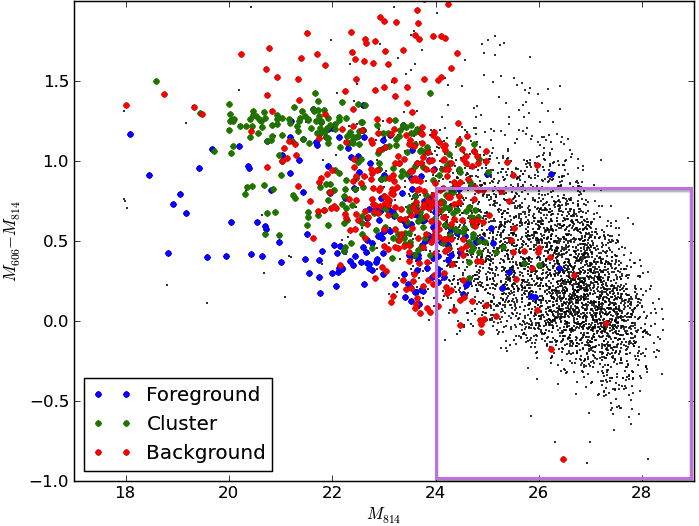
\includegraphics[width=4in]{Chapter2/HSTcolormag_wBPZ.png}
\caption[Musket Ball Cluster color-magnitude diagram based on HST photometry, along with galaxy location based on DLS photometric redshifts.]{Musket Ball Cluster color-magnitude diagram based on HST photometry.  The larger color points are cross-matched DLS objects which have been divided into \emph{Foreground} (blue; $z_{\rm phot}<0.43$), \emph{Cluster} (green; $z_{\rm phot}=0.53\pm0.1$), and \emph{Background} (red; $z_{\rm phot}>0.63$) samples.  Note that the photometric redshifts become relatively unreliable for $M_{\rm 814}>24$. 
The purple box indicates the HST source galaxy sample.  
\label{figure:HSTcolormag}}
\end{figure}

\begin{figure}
\centering
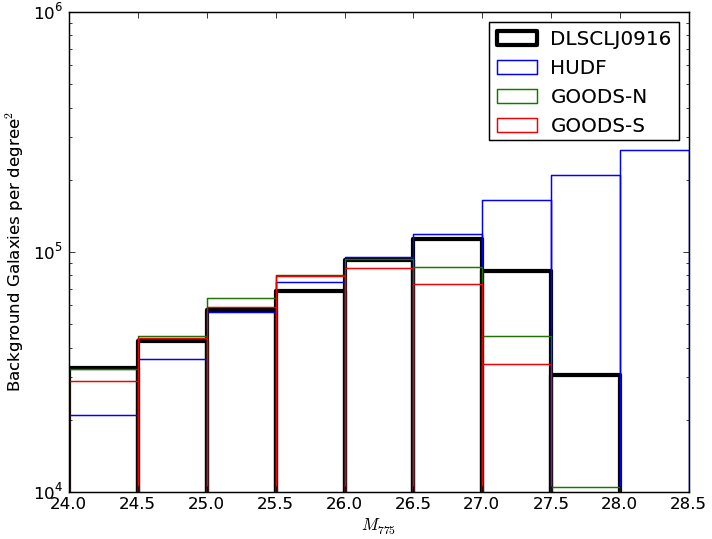
\includegraphics[width=4in]{Chapter2/UDF_GOODS_sourcemaghist.png}
\caption[Comparison of the Musket Ball Cluster, HUDF and GOODS North \& South source galaxy densities.]{Comparison of the Musket Ball Cluster, HUDF \citep{Coe:2006jf} and GOODS North \& South \citep{Giavalisco:2004kl} source galaxy densities.
The HUDF field has a depth of 288 F775W orbits, the GOODS survey has a depth of one F775W orbit, and the Musket Ball Cluster has a depth of 2 F814W orbits (the F814W filter is conservatively wider than the F775W filter).
Up to the completeness of each survey we find a comparable number distribution of sources as a function of magnitude when we make similar cuts to each galaxy catalog, indicating negligible cluster contamination.
\label{figure:HSTsourcedensity}}
\end{figure}

We construct a joint catalog from the HST and Subaru data, using the HST data where available and Subaru for the surrounding area.
Using a tomography-based MCMC analysis we simultaneously fit NFW halos centered on the North and South HST WL peaks, and use the \citet{Gelman:1992ht} convergence test applied to eight independent chains.
In order to reduce the number of free parameters we use the \citet{Duffy:2008jy} empirical relation between $M_{200}$ and concentration.
We present the most likely masses for each halo along with the bias-corrected 68\% confidence limits in Table \ref{tbl1}.
We also compare the integrated projected surface mass density of the NFW halos with the measured WL aperture mass \citep{Fahlman:1994eb} of each subcluster and find agreement within a radius of 0.5 Mpc of each subcluster.

\begin{figure}
%\plottwo{fig3a.eps}{fig3b.eps}
\plotone{Chapter2/fig3.png}
\caption[Comparison of the Subaru $i'$-band ground-based and HST space-based  WL mass signal-to-noise maps of DLSCL J0916.2+2951 with the X-ray distribution and galaxy number density.]{Comparison of the Subaru $i'$-band ground-based (left) and HST space-based (right) WL mass signal-to-noise maps (color) of DLSCL J0916.2+2951 with the X-ray distribution (bold black contours) and galaxy number density (white contours, same as Figure \ref{fig2}). The peak centers and corresponding one sigma errors are denoted by the gray cross-hairs.
In both analyses there is agreement between the location and relative magnitude of galaxies and WL yet the majority of the cluster gas is centered $\sim1.4\arcmin$ between the North and South subclusters in a local mass underdensity, providing evidence that the North and South subclusters have undergone the first pass-through of a major merger.
The scale of each map is equivalent and the image field-of-view is the same as Figures \ref{fig1} \& \ref{fig2}.
The map created from the joint Subaru/HST catalog looks nearly identical to the HST map, with only slight variations in the scale (see Table \ref{tbl1}).
\label{fig3}}
\end{figure}

\section{Sunyaev--Zel'dovich Effect Studies}

This cluster was also observed in the Sunyaev-Zel'dovich Array Survey \citep{Muchovej:2010gc}.  
They found a 4{$\sigma$} SZE signal roughly consistent with that expected for clusters of this mass.
The signal is offset $\sim$ 1' ($\sim$ 0.4 Mpc) from the southern subcluster and $\sim$ 3' ($\sim$ 1 Mpc) from the northern subcluster.
The SZE traces the cluster ICM and can be used to identify an offset of the ICM relative to the galaxies and dark matter \citep[as in the case of the Bullet Cluster][]{Halverson:2009gn}.
This shift provided the first evidence that the cluster gas is dissociated from the bulk of the mass and galaxies (Figure \ref{figure:MusketBallSZ}).

\begin{figure}
\centering
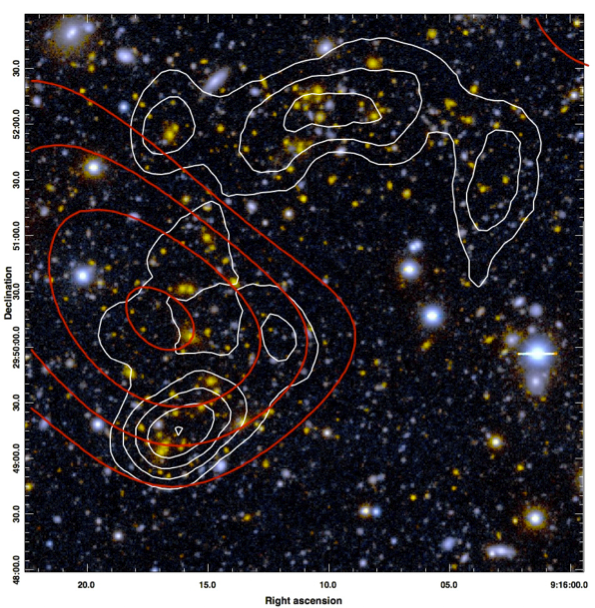
\includegraphics[width=4in]{Chapter2/color_2contours_noblue_edit.png}
\caption[DLS optical image with SZE and galaxy number density maps.]{DLS composite $BVR$ color image of DLSCL J0916.2+2951 showing evidence that the cluster gas, represented by the solid red SZE decrement significance contours (1, 2, 3, 4$\sigma$), is offset $\sim1\arcmin$ ($\sim0.4$ Mpc) and $\sim3\arcmin$ ($\sim1$ Mpc) from the two subclusters, represented by the white galaxy number density contours for galaxies with $z_{\rm phot}=0.53\pm0.1$ (beginning at 200 galaxies\,Mpc$^{-2}$ with increments of 50). 
The image field-of-view is the same as Figure \ref{fig1}. 
The beam of the SZ observation has a radius of $\sim1\arcmin$.\label{figure:MusketBallSZ}}
\end{figure}

\section{X-ray Studies}

We acquired X-ray spectral-imaging of the cluster with 40ks of {\it Chandra} ACIS-I time (GO-12800854, PI Dawson), and reduce it using \emph{CIAO} version 4.2 and \emph{CALDB} version 4.4.1.
We manually identify X-ray point sources and mask them before adaptively smoothing the diffuse emission, we present the resulting map in Figure \ref{figure:MusketBallXray}.
We estimate source counts and their error using the \emph{dmextract} function of \emph{CIAO}.
We use an 8$\arcmin$ radius background region which encloses the subcluster regions and rests $\sim90\%$ on ACIS-I3 (on which the subclusters are observed).
In the estimate of the background counts each subcluster region, chip gap, and point source are excluded.
The subcluster exclusion regions were defined such that they encompassed the source emission and were extended out to approximately the SNR = 1 level based on the smoothed map.
In total we there were $1800\pm40$ background counts in 620,000 pixel$^2$ area within the energy range of 0.5-2\,keV.
For the South and Central X-ray concentrations (120$\pm$17 and 170$\pm$19 detected 0.5-2\,keV photons, respectively) we use the \emph{Xspec} X-ray spectral fitting tool \citep{Arnaud:1996vl} to fit a Mewe-Kaastra-Liedahl plus photoelectric absorption model \citep[fixed to the Leiden/Argentine/Bonn value;][]{Kalberla:2005de} to the X-ray spectrum of each X-ray concentration.
For the North concentration there are not enough detected X-ray photons (38$\pm$12) to fit a meaningful spectrum.  
We report the results of this analysis in Table \ref{tbl1}. 
We define the subcluster exclusion regions such that they encompass the source emission and extend out to approximately the 1$\sigma$ level based on the smoothed map.  
In total there are $1800\pm40$ background counts in the 620,000\,pixel$^2$ area and 0.5-2\,keV energy range.
For the North, South, and Central X-ray concentrations we find 38$\pm$12, 120$\pm$17 and 170$\pm$19 detected 0.5-2\,keV photons, respectively.   
 
To estimate the temperatures of the South and Central concentrations we use the \emph{Xspec} X-ray spectral fitting tool \citep{Arnaud:1996vl} to fit a Mewe-Kaastra-Liedahl plus photoelectric absorption model \citep[fixed to the Leiden/Argentine/Bonn value;][]{Kalberla:2005de} to the X-ray spectrum of each X-ray concentration.  
For the North concentration there are not enough detected X-ray photons to fit a meaningful spectrum.  
Due to the low count regime and our use of the $\chi^2$ statistic we rebin the data so that each spectral channel used in the fit contains at least 20 counts.
The binning is carried out on the spectra before background subtraction; these raw spectra contained 843 (1070) counts in the South (Central) subcluster.
Since the background spectrum contains 7725 counts, each spectral bin in the background is far above the 20 count threshold.
Binning data in this manner does reduce the spectral resolution, however for hot clusters like those in our study the number of final spectral bins we have (31 for the southern and 39 for the central subcluster, which include cuts on the highest energy channels) are sufficient to determine the temperature, since the spectrum is dominated by bremsstrahlung emission which has few sharp spectral features. 
We report the results of this analysis in Table \ref{tbl1}.

\begin{figure}
\centering
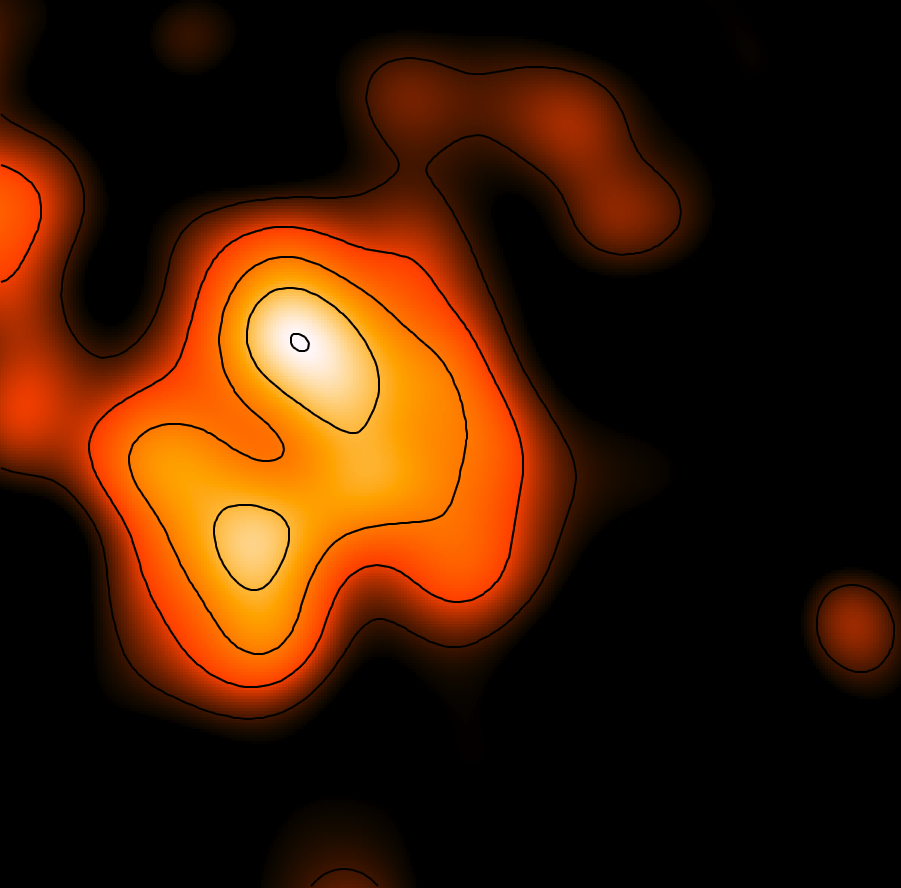
\includegraphics[width=4in]{Chapter2/XrayMapwithContours.png}
\caption[X-ray map of the Musket Ball Cluster]{
Chandra ACIS-I 40\,ks adaptively smoothed X-ray image of DLSCL J0916.2+2951.
The image field-of-view is the same as Figure \ref{fig1}.
The contours are evenly spaced on an arbitrary linear scale and are used throughout this dissertation when comparing the gas map with other components.
\label{figure:MusketBallXray}}
\end{figure}

\section{Radio Studies}

Since the Musket Ball cluster is a strong merger with an X-ray inferred\footnote{The estimated Mach number is based on the X-ray temperature of the gas (Table \ref{tbl1}) and estimated collision velocity of the merger (Table \ref{musketballresultparam}).} Mach number of $>$ 3 whose axis is likely to be close to the plane of the sky \citep[][and presented in Chapter \ref{chapter:3}]{Dawson:2012ub}, it is a prime candidate for a double radio relic. 
Radio relics are irregularly shaped radio sources, located at the outskirts of galaxy clusters, characterized by a steep radio spectrum\footnote{The spectrum is defined as $S(\nu)\propto\nu^\alpha$.} with $\alpha\leq -1.2$.
Radio relics are thought to be produced by relativistic particles that have been accelerated by shock waves in the ICM.
Double relics show relics on opposite sides from the cluster center and form a subset of relics for which the merger geometry can be constrained particularly well \citep[see e.g.][]{Bonafede:2012fu}.

Since the Musket Ball Cluster is at a later stage than all other dissociative
mergers \citep{Dawson:2012dl} and is thought to have shocks with $M >
3$, the detection of radio relics would provide constraints on the merger geometry. 
This has direct implications for the measurement of the dark matter cross-section with the Musket Ball since observed projected offsets must be translated into meaningful physical offsets \citep[see e.g.][]{Dawson:2012ub}. 
The degree of polarization provides important information on the angle of the shock surface and the line of sight and together with the location of the relics with respect to the X-ray position we can constrain the geometry of the merger axis to within 10 degrees \citep{vanWeeren:2011cd}. 
Furthermore, the cluster makes an ideal target to study the evolution of radio relics, due to its superior temporal lever arm, with ramifications for the theory of particle acceleration. 

The Musket Ball Cluster is located at $z$ = 0.53 and at this redshift a typical moderate luminosity radio relic has a flux density of 0.3 mJy at $z$ = 0.53 and 1.4 GHz \citep{Nuza:2012fu, vanWeeren:2011cd}. 
This is well below both the NRAO VLA Sky Survey (NVSS) and Westerbork Northern Sky Survey (WENNS) sensitivities, thus an existing non-detection in these surveys is not surprising. 

We observed the Musket Ball Cluster with the Westerbork Synthesis Radio Telescope (WSRT) in 2013 January 23-28 for a total of 24 hours.  We used the standard 21\,cm L-band as it is the most sensitive system at the WSRT.
The observations have a resolution of about 15x30 arcsec, corresponding to a physical size of 100x200kpc at z = 0:53, enough to resolve a 1 Mpc relic (relic sizes range between 0.5 and 2 Mpc).
With two full synthesis runs we achieved a noise level of 20\,$\mu$Jy/beam in the continuum, and about 10\,$mu$Jy/beam in Stokes Q and U. 
This should enable us to detect a 0.3\,mJy relic, covering 5 beam areas, with
an SNR of 10. 

While there are a number of compact sources associated with the merging cluster (see the $X$'s in Figure \ref{figure:MusketBallRadio}), we find no evidence for diffuse radio emission associated with the merging cluster.
In other words, no radio halos or relics are detected in the Musket Ball Cluster merger.
All previously discovered radio relics have been in clusters with X-ray luminosities in the range of 10$^{44}$-10$^{45}$\,erg\,s$^{-1}$.
The Musket Ball Cluster has an X-ray luminosity of $\sim 10^{43}$\,erg\,s$^{-1}$ (see Table \ref{tbl1}). 
This null detection is in line with current observations suggesting that radio relics are only found in very massive cluster mergers, although without better measurements of the cluster merger velocity and gas sound speed there remains the possibility that the merger Mach number $\gtrsim$ 3 is an overestimate.

\begin{figure}
\centering
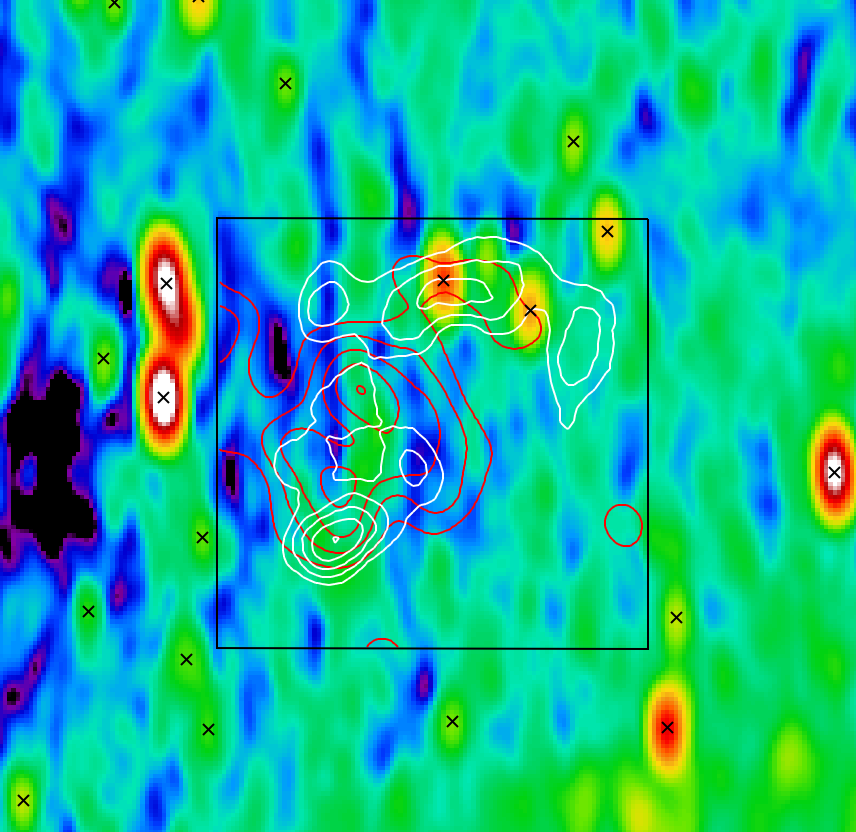
\includegraphics[width=4in]{Chapter2/RadioWithGalaxyAndXrayContours.png}
\caption[Radio survey of the Musket Ball Cluster and surrounding area.]{
Westerbork Synthesis Radio Telescope 21cm L-band image of the Musket Ball Cluster and surrounding area.  The color image has an arbitrary log-scale.  Likely compact radio sources are denoted by the \emph{X} points, and from these the north/south elongated PSF can be seen.  The black box shows the area corresponding to Figures \ref{fig1}, \ref{fig2}, and \ref{fig3}. Similarly the white contours are the galaxy number density contours from Figure \ref{fig2}, and the red contours are the X-ray contours from Figure \ref{fig3}.  We detect no significant diffuse radio emission associated with the Musket Ball Cluster (i.e. no radio halos or relics are detected).
\label{figure:MusketBallRadio}}
\end{figure}

\section{Cluster Merger Scenario}

The peak of the gas distribution ($09\fh16\fm15\fs\pm5.5\fs, 29\fdg50\farcm59\farcs\pm5.0\farcs$) derived from X-rays is offset $1.4\arcmin\pm0.49$ from the North HST WL mass peak ($09\fh16\fm10\fs\pm30\fs, 29\fdg52\farcm10\farcs\pm30\farcs$), and $1.4\arcmin\pm0.14$ from the South HST WL mass peak ($09\fh16\fm15\fs\pm8.0\fs, 29\fdg49\farcm34\farcs\pm6.9\farcs$), and is located near a local minimum in the mass, suggesting that the subclusters have a small impact parameter and have experienced at least their first pass-through along a north-northwest merger direction (see Figure \ref{fig3}).
Additionally the central X-ray concentration has a temperature (Table \ref{tbl1}) in line with an M$_{500}=0.9^{+1.1}_{-0.3}\times10^{14}$\,M$_{\odot}$ potential \citep{Vikhlinin:2009jy}, but the WL data suggests that there is a local under-density of mass at this concentration incapable of supporting such a temperature.
Further evidence for the merger scenario is provided by the morphology of the gas.
Simulations \citep{Schindler:1993vl,Poole:2006gp} predict that the gas morphology elongates transverse to the merger direction after pass-through for mergers with small impact parameters.
The Central gas concentration appears to be oblate and roughly perpendicular to the axis connecting the North and South mass peaks.
This is consistent with the interpretation that these two subclusters have experienced their first pass-through and that the merger axis being roughly in the plane of the sky.

\section{Discussion}

While we use DLSCL J0916.2+2951 to provide further evidence for the canonical DM model and independently constrain $\sigma_{\rm DM}m^{-1}_{\rm DM}$, we believe that its greatest value is as a probe for a new and special phase of cluster formation.  
It provides a greatly improved temporal lever-arm with which to guide numerical simulations that explore the major merger phase.  
This is potentially important given that much of our knowledge of the cluster merger process comes from numerical hydrodynamic simulations \cite[e.g.][]{Poole:2006gp}, which are used to place the tightest constraints on $\sigma_{\rm DM}m^{-1}_{\rm DM}$ \citep[$<0.7$\,cm$^2$\,g$^{-1}$;][]{Randall:2008hs} and bring observed merger velocities (inferred from the observed shock velocity) more in line with the expectations of $\Lambda$CDM \citep{Springel:2007bg,Lee:2010id}.
Secondly, the large projected separation relative to the virial radii of the subclusters ($R_{200} \sim 1$Mpc) enables the deconvolution of the subclusters from the Central region and direct comparison of the physical properties of each.
This will provide new insight into the behavior of the cluster constituents (gas, galaxies, \& DM) during a major merger.
For example, it is well established that galaxy clusters play an important role in the evolution of their member galaxies, but it is still unclear whether cluster mergers trigger star formation \citep[e.g.][]{Miller:2003kx,Owen:2005dx,Ferrari:2005es,Hwang:2009ip}, quench it \citep{Poggianti:2004ca}, or have no immediate effect \citep{Chung:2010ds}.

Our identification of DLSCL J0916.2+2951 as a dissociative merging system using only optical, WL, and SZE observations shows that these systems can be found independent of X-ray observations.
This has implications for finding more of these systems when the existing SZE surveys, e.g. ACT \citep{Hincks:2010ff} and SPT \citep{Ruhl:2004io}, are coupled with upcoming and overlapping deep optical/WL surveys, e.g. DES \citep{Collaboration:2005vv} and LSST \citep{Tyson:2002hn}.

\noindent\textbf{acknowledgements:}

We thank Daniel P. Marrone, Stephen Muchovej,  John E. Carlstrom, and Tony Mroczkowski of the SZA collaboration for sharing the results of the SZA Survey, which helped motivate the detailed follow-up campaign of DLSCL J0916.2+2951. 
Support for this work was provided by NASA through Chandra Award Number GO1-12171X issued by CXO Center, which is operated by the SAO for and on behalf of NASA under contract NAS8-03060.  Support for program number GO-12377 was provided by NASA through a grant from STScI, which is operated by the Association of Universities for Research in Astronomy, Inc., under NASA contract NAS5-26555.

This work made use of the following facilities: CXO (ACIS-I), HST (ACS), Keck:I (LRIS), Keck:2 (DEIMOS), Mayall (MOSAIC 1 \& 1.1), Subaru (Suprime-Cam), SZA.
